\chapter{Introduction}\label{chap:chap0}

\epigraph{Awesome citation}{Awesome author}
\clearpage

\lettrine[lines=2, lraise=0., nindent=0em, slope=-.5em]%
{T}{he} problem of humanoid walk planning can be defined as follows:
given an environment and a humanoid robot with start and goal
placements, a collision-free trajectory needs to be found. It should
ideally represent realistic human motion, i.e. a motion similar to
that of a human being in the same conditions. This result is desirable
since humanoid robots are bound to move in man-made environments such
as homes, offices, and factories and because it can help them blend in
among humans.

\begin{figure}
  \centering
      {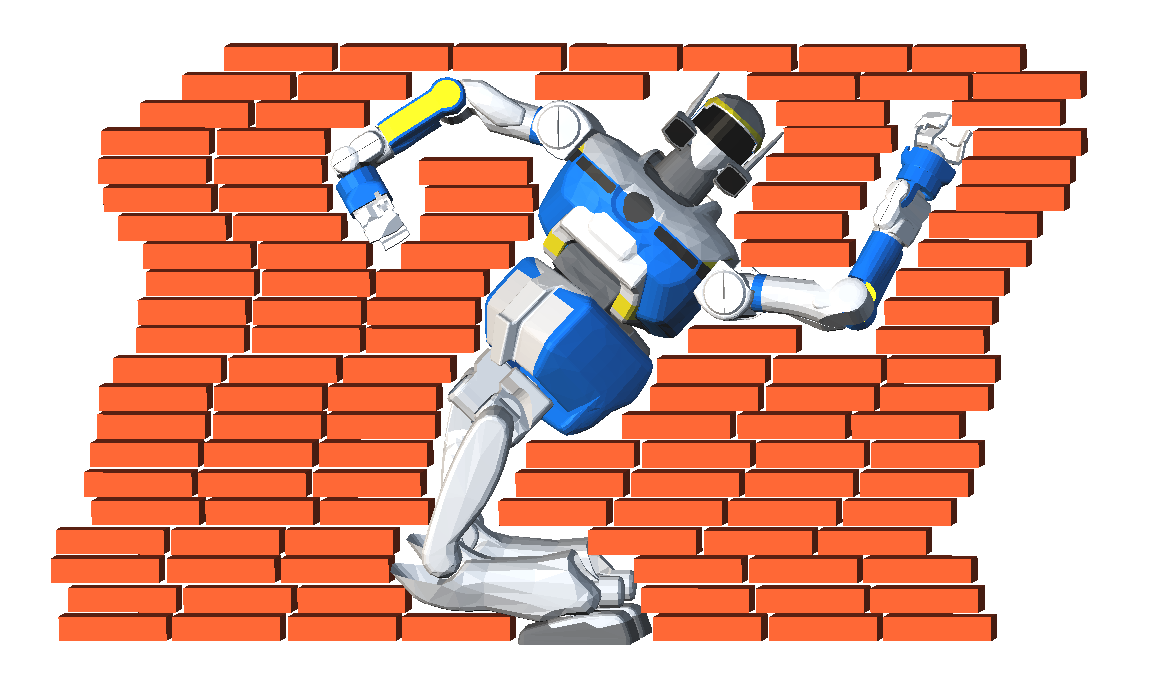
\includegraphics[width = 0.9\linewidth]
        {src/chap1-path-optimization/hrp2-brick-wall.png}}
      \caption{FIXME: redundant and underactuated system: humanoid
        robot, + obstacle avoidance}
      \label{fig:chap0-hrp2-brick-wall}
\end{figure}

\section[Contributions]{Contributions}

Chapter \autoref{chap:path-optim} deals with humanoid walk planning in
cluttered environments. It presents a heuristic and efficient
optimization method that takes as input a path computed for the robot
bounding box, and produces a path where a discrete set of
configurations is reoriented using an A* search algorithm. The
resulting trajectory is realistic and time-optimal. This method is
validated in various scenarios on the humanoid robot HRP-2.

http://www.willowgarage.com/blog/2009/09/04/robot-comics-path-planning


